\scanpage{53}
% L01-07
\uline{Dém} $s_1\ne s_0$ \inserted{et $s_2\ne s_0$} par a) 1°; $a_1\ne a_0$ par b), donc $s_2\notin a_0$, donc $s_0,s_1,s_2$ aff\textsuperscript{t} indép, $f_0$ est le plan qu'ils engendrent. \unsure{De m} \unsure{(en remplaçant|[remplaçant} \inserted{$r_0=(s_0,a_0,f_0)$} par $r_1=(s_0,a_0,f_1)$] on voit que $f_1$ est le plan engendré par $s_0,s_1,s_{\unsure{2|3}}$. Or $f_1\ne f_0$ \deleted{\unsure{(car|(par|par}} par a) 2°, donc $s_3\notin f_0$, donc $s_0,s_1,s_2,s_3$ aff\textsuperscript{t} indép.

% L08-10
\uline{Cor}
\[
\begin{aligned}
a_0&=\mathrm{dr}(s_0,s_1)\\
f_0&=\mathrm{pl}(s_0,s_1,s_2)
\end{aligned}
\mathrel{\big|\!\!\Longrightarrow}
\begin{gathered}
\varphi_A,\varphi_F\ \text{connus quand}\\
\text{on \unsure{connaît|connait} }\varphi_S
\end{gathered}
\]

% L11-15
\unsure{de même}
\[
\begin{aligned}
a_0&=f_0\cap f_1\\
s_0&=f_0\cap f_1\cap f_2
\end{aligned}
\mathrel{\big|\!\!\Longrightarrow}
\begin{gathered}
\varphi_S,\varphi_A\ \text{connus}\\
\text{quand on}\\
\text{\unsure{connaît|connait} }\varphi_F
\end{gathered}
\]
où $f_2$ est la deuxième face passant par $a_1$

% Lower-left drawing, alongside L16-18
\figure{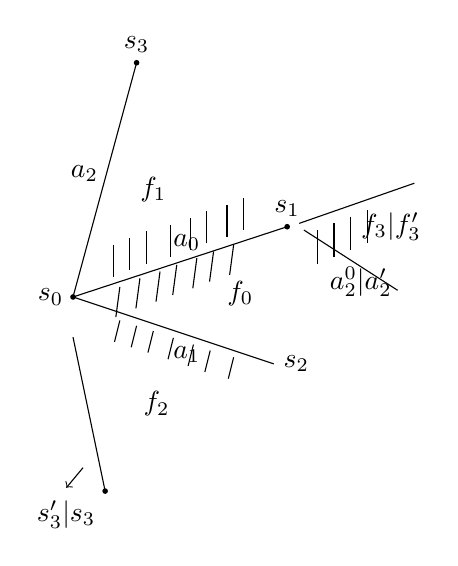
\begin{tikzpicture}[scale=.85]
\coordinate (s0) at (0,0);
\coordinate (s1) at (3.2,1.05);
\coordinate (s2) at (3,-1);
\coordinate (s3) at (.95,3.5);
\coordinate (s3b) at (.48,-2.9);
\draw (s3)--(s0)--(s1);
\draw (3.38,1.1)--(5.1,1.7);
\draw (3.45,1.0)--(4.85,.1);
\draw (s0)--(s2);
\draw (0,-.6)--(s3b);
\foreach \x/\y in {.6/.3,.85/.4,1.1/.5,1.45/.6,1.75/.7,2/.8,2.3/.9,2.55/1.0}
 {\draw[thin] (\x,\y)--+(0,.48);}
\foreach \x/\y in {.7/.15,1/.28,1.3/.38,1.55/.48,1.85/.58,2.1/.68,2.4/.78}
 {\draw[thin] (\x,\y)--+(-.06,-.45);}
\foreach \x/\y in {.7/-.35,.95/-.43,1.2/-.51,1.5/-.61,1.8/-.71,2.05/-.8,2.4/-.9}
 {\draw[thin] (\x,\y)--+(-.08,-.32);}
\foreach \x/\y in {3.65/1.0,3.9/1.1,4.15/1.2,4.4/1.3}
 {\draw[thin] (\x,\y)--+(0,-.5);}
\fill (s0) circle (1.2pt) (s1) circle (1.2pt) (s3) circle (1.2pt) (s3b) circle (1.2pt);
\node[left] at (s0) {$s_0$}; \node[above] at (s1) {$s_1$};
\node[right] at (s2) {$s_2$}; \node[above] at (s3) {$s_3$};
\node[below left] at (s3b) {$\unsure{s'_3|s_3}$};
\draw[->] (.15,-2.55)--(-.1,-2.85);
\node[above] at (1.7,.55) {$a_0$}; \node[below] at (1.7,-.6) {$a_1$};
\node[left] at (.52,1.85) {$a_2$}; \node[below] at (4.3,.6) {$\unsure{a_2^0|a_2'}$};
\node at (2.5,.05) {$f_0$}; \node at (1.2,1.6) {$f_1$};
\node at (1.25,-1.6) {$f_2$}; \node at (4.75,1.05) {$\unsure{f_3|f'_3}$};
\end{tikzpicture}}

% L16-18, right of drawing
et enfin
\[
\begin{aligned}
s_0&=a_0\cap a_1\\
f_0&=\mathrm{pl}(a_0,a_1)
\end{aligned}
\mathrel{\big|\!\!\Longrightarrow}
\begin{gathered}
\varphi_S,\varphi_F\ \text{connus}\\
\text{quand on}\\
\text{\unsure{connaît|connait} }\varphi_A
\end{gathered}
\]

% L19
\uline{Corollaire} $\unsure{S|\mathscr{S}}=\varphi_S(\underline{S})$ engendre aff\textsuperscript{t} $E$.

% L20-21
Réalisation géom \uline{régulière} (si $\underline{X}$ \uline{régulier})
\[
\forall\underline{g}\in\underline{\unsure{G|C}}\overset{\unsure{\mathrm{df}|\mathrm{déf}}}{=}\mathrm{Aut}(X),\quad
\exists g\in\mathrm{Aut}_{\text{aff ou proj}}(E)
\]
% archive sheet number: 52
